

\tikzset{every picture/.style={line width=0.75pt}} %set default line width to 0.75pt        

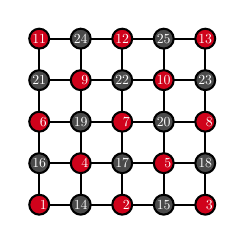
\begin{tikzpicture}[x=0.75pt,y=0.75pt,yscale=-1,xscale=1]
%uncomment if require: \path (0,222); %set diagram left start at 0, and has height of 222

%Shape: Grid [id:dp7509010194001084] 
\draw  [draw opacity=0][fill={rgb, 255:red, 255; green, 255; blue, 255 }  ,fill opacity=1 ] (289.5,76) -- (369.67,76) -- (369.67,156.5) -- (289.5,156.5) -- cycle ; \draw   (289.5,76) -- (289.5,156.5)(309.5,76) -- (309.5,156.5)(329.5,76) -- (329.5,156.5)(349.5,76) -- (349.5,156.5)(369.5,76) -- (369.5,156.5) ; \draw   (289.5,76) -- (369.67,76)(289.5,96) -- (369.67,96)(289.5,116) -- (369.67,116)(289.5,136) -- (369.67,136)(289.5,156) -- (369.67,156) ; \draw    ;
%Shape: Circle [id:dp6108755291859196] 
\draw  [fill={rgb, 255:red, 208; green, 2; blue, 27 }  ,fill opacity=1 ] (284.71,156) .. controls (284.71,153.35) and (286.85,151.21) .. (289.5,151.21) .. controls (292.15,151.21) and (294.29,153.35) .. (294.29,156) .. controls (294.29,158.65) and (292.15,160.79) .. (289.5,160.79) .. controls (286.85,160.79) and (284.71,158.65) .. (284.71,156) -- cycle ;
%Shape: Circle [id:dp4441687082516983] 
\draw  [fill={rgb, 255:red, 74; green, 74; blue, 74 }  ,fill opacity=1 ] (304.71,156) .. controls (304.71,153.35) and (306.85,151.21) .. (309.5,151.21) .. controls (312.15,151.21) and (314.29,153.35) .. (314.29,156) .. controls (314.29,158.65) and (312.15,160.79) .. (309.5,160.79) .. controls (306.85,160.79) and (304.71,158.65) .. (304.71,156) -- cycle ;
%Shape: Circle [id:dp6167896316379069] 
\draw  [fill={rgb, 255:red, 208; green, 2; blue, 27 }  ,fill opacity=1 ] (324.71,156) .. controls (324.71,153.35) and (326.85,151.21) .. (329.5,151.21) .. controls (332.15,151.21) and (334.29,153.35) .. (334.29,156) .. controls (334.29,158.65) and (332.15,160.79) .. (329.5,160.79) .. controls (326.85,160.79) and (324.71,158.65) .. (324.71,156) -- cycle ;
%Shape: Circle [id:dp6715236044117903] 
\draw  [fill={rgb, 255:red, 74; green, 74; blue, 74 }  ,fill opacity=1 ] (344.71,156) .. controls (344.71,153.35) and (346.85,151.21) .. (349.5,151.21) .. controls (352.15,151.21) and (354.29,153.35) .. (354.29,156) .. controls (354.29,158.65) and (352.15,160.79) .. (349.5,160.79) .. controls (346.85,160.79) and (344.71,158.65) .. (344.71,156) -- cycle ;
%Shape: Circle [id:dp06410493254248473] 
\draw  [fill={rgb, 255:red, 208; green, 2; blue, 27 }  ,fill opacity=1 ] (364.71,156) .. controls (364.71,153.35) and (366.85,151.21) .. (369.5,151.21) .. controls (372.15,151.21) and (374.29,153.35) .. (374.29,156) .. controls (374.29,158.65) and (372.15,160.79) .. (369.5,160.79) .. controls (366.85,160.79) and (364.71,158.65) .. (364.71,156) -- cycle ;
%Shape: Circle [id:dp6649764858783351] 
\draw  [fill={rgb, 255:red, 208; green, 2; blue, 27 }  ,fill opacity=1 ] (364.71,116) .. controls (364.71,113.35) and (366.85,111.21) .. (369.5,111.21) .. controls (372.15,111.21) and (374.29,113.35) .. (374.29,116) .. controls (374.29,118.65) and (372.15,120.79) .. (369.5,120.79) .. controls (366.85,120.79) and (364.71,118.65) .. (364.71,116) -- cycle ;
%Shape: Circle [id:dp9554900297815432] 
\draw  [fill={rgb, 255:red, 74; green, 74; blue, 74 }  ,fill opacity=1 ] (364.71,136) .. controls (364.71,133.35) and (366.85,131.21) .. (369.5,131.21) .. controls (372.15,131.21) and (374.29,133.35) .. (374.29,136) .. controls (374.29,138.65) and (372.15,140.79) .. (369.5,140.79) .. controls (366.85,140.79) and (364.71,138.65) .. (364.71,136) -- cycle ;
%Shape: Circle [id:dp37112581806137124] 
\draw  [fill={rgb, 255:red, 208; green, 2; blue, 27 }  ,fill opacity=1 ] (344.71,136) .. controls (344.71,133.35) and (346.85,131.21) .. (349.5,131.21) .. controls (352.15,131.21) and (354.29,133.35) .. (354.29,136) .. controls (354.29,138.65) and (352.15,140.79) .. (349.5,140.79) .. controls (346.85,140.79) and (344.71,138.65) .. (344.71,136) -- cycle ;
%Shape: Circle [id:dp06306680838602707] 
\draw  [fill={rgb, 255:red, 74; green, 74; blue, 74 }  ,fill opacity=1 ] (324.71,136) .. controls (324.71,133.35) and (326.85,131.21) .. (329.5,131.21) .. controls (332.15,131.21) and (334.29,133.35) .. (334.29,136) .. controls (334.29,138.65) and (332.15,140.79) .. (329.5,140.79) .. controls (326.85,140.79) and (324.71,138.65) .. (324.71,136) -- cycle ;
%Shape: Circle [id:dp9358022961380756] 
\draw  [fill={rgb, 255:red, 208; green, 2; blue, 27 }  ,fill opacity=1 ] (304.71,136) .. controls (304.71,133.35) and (306.85,131.21) .. (309.5,131.21) .. controls (312.15,131.21) and (314.29,133.35) .. (314.29,136) .. controls (314.29,138.65) and (312.15,140.79) .. (309.5,140.79) .. controls (306.85,140.79) and (304.71,138.65) .. (304.71,136) -- cycle ;
%Shape: Circle [id:dp9068520178890649] 
\draw  [fill={rgb, 255:red, 74; green, 74; blue, 74 }  ,fill opacity=1 ] (284.71,136) .. controls (284.71,133.35) and (286.85,131.21) .. (289.5,131.21) .. controls (292.15,131.21) and (294.29,133.35) .. (294.29,136) .. controls (294.29,138.65) and (292.15,140.79) .. (289.5,140.79) .. controls (286.85,140.79) and (284.71,138.65) .. (284.71,136) -- cycle ;
%Shape: Circle [id:dp8562155796812134] 
\draw  [fill={rgb, 255:red, 208; green, 2; blue, 27 }  ,fill opacity=1 ] (284.71,116) .. controls (284.71,113.35) and (286.85,111.21) .. (289.5,111.21) .. controls (292.15,111.21) and (294.29,113.35) .. (294.29,116) .. controls (294.29,118.65) and (292.15,120.79) .. (289.5,120.79) .. controls (286.85,120.79) and (284.71,118.65) .. (284.71,116) -- cycle ;
%Shape: Circle [id:dp2479839382803859] 
\draw  [fill={rgb, 255:red, 74; green, 74; blue, 74 }  ,fill opacity=1 ] (304.71,116) .. controls (304.71,113.35) and (306.85,111.21) .. (309.5,111.21) .. controls (312.15,111.21) and (314.29,113.35) .. (314.29,116) .. controls (314.29,118.65) and (312.15,120.79) .. (309.5,120.79) .. controls (306.85,120.79) and (304.71,118.65) .. (304.71,116) -- cycle ;
%Shape: Circle [id:dp8339992993489453] 
\draw  [fill={rgb, 255:red, 208; green, 2; blue, 27 }  ,fill opacity=1 ] (324.71,116) .. controls (324.71,113.35) and (326.85,111.21) .. (329.5,111.21) .. controls (332.15,111.21) and (334.29,113.35) .. (334.29,116) .. controls (334.29,118.65) and (332.15,120.79) .. (329.5,120.79) .. controls (326.85,120.79) and (324.71,118.65) .. (324.71,116) -- cycle ;
%Shape: Circle [id:dp29657132974437017] 
\draw  [fill={rgb, 255:red, 74; green, 74; blue, 74 }  ,fill opacity=1 ] (344.71,116) .. controls (344.71,113.35) and (346.85,111.21) .. (349.5,111.21) .. controls (352.15,111.21) and (354.29,113.35) .. (354.29,116) .. controls (354.29,118.65) and (352.15,120.79) .. (349.5,120.79) .. controls (346.85,120.79) and (344.71,118.65) .. (344.71,116) -- cycle ;
%Shape: Circle [id:dp4006844726389853] 
\draw  [fill={rgb, 255:red, 74; green, 74; blue, 74 }  ,fill opacity=1 ] (284.71,96) .. controls (284.71,93.35) and (286.85,91.21) .. (289.5,91.21) .. controls (292.15,91.21) and (294.29,93.35) .. (294.29,96) .. controls (294.29,98.65) and (292.15,100.79) .. (289.5,100.79) .. controls (286.85,100.79) and (284.71,98.65) .. (284.71,96) -- cycle ;
%Shape: Circle [id:dp2518725902881924] 
\draw  [fill={rgb, 255:red, 208; green, 2; blue, 27 }  ,fill opacity=1 ] (304.71,96) .. controls (304.71,93.35) and (306.85,91.21) .. (309.5,91.21) .. controls (312.15,91.21) and (314.29,93.35) .. (314.29,96) .. controls (314.29,98.65) and (312.15,100.79) .. (309.5,100.79) .. controls (306.85,100.79) and (304.71,98.65) .. (304.71,96) -- cycle ;
%Shape: Circle [id:dp9478829895408571] 
\draw  [fill={rgb, 255:red, 74; green, 74; blue, 74 }  ,fill opacity=1 ] (324.71,96) .. controls (324.71,93.35) and (326.85,91.21) .. (329.5,91.21) .. controls (332.15,91.21) and (334.29,93.35) .. (334.29,96) .. controls (334.29,98.65) and (332.15,100.79) .. (329.5,100.79) .. controls (326.85,100.79) and (324.71,98.65) .. (324.71,96) -- cycle ;
%Shape: Circle [id:dp5111042484735311] 
\draw  [fill={rgb, 255:red, 208; green, 2; blue, 27 }  ,fill opacity=1 ] (344.71,96) .. controls (344.71,93.35) and (346.85,91.21) .. (349.5,91.21) .. controls (352.15,91.21) and (354.29,93.35) .. (354.29,96) .. controls (354.29,98.65) and (352.15,100.79) .. (349.5,100.79) .. controls (346.85,100.79) and (344.71,98.65) .. (344.71,96) -- cycle ;
%Shape: Circle [id:dp08226041749176072] 
\draw  [fill={rgb, 255:red, 74; green, 74; blue, 74 }  ,fill opacity=1 ] (364.71,96) .. controls (364.71,93.35) and (366.85,91.21) .. (369.5,91.21) .. controls (372.15,91.21) and (374.29,93.35) .. (374.29,96) .. controls (374.29,98.65) and (372.15,100.79) .. (369.5,100.79) .. controls (366.85,100.79) and (364.71,98.65) .. (364.71,96) -- cycle ;
%Shape: Circle [id:dp6793036732090996] 
\draw  [fill={rgb, 255:red, 208; green, 2; blue, 27 }  ,fill opacity=1 ] (284.71,76) .. controls (284.71,73.35) and (286.85,71.21) .. (289.5,71.21) .. controls (292.15,71.21) and (294.29,73.35) .. (294.29,76) .. controls (294.29,78.65) and (292.15,80.79) .. (289.5,80.79) .. controls (286.85,80.79) and (284.71,78.65) .. (284.71,76) -- cycle ;
%Shape: Circle [id:dp4959600894339744] 
\draw  [fill={rgb, 255:red, 74; green, 74; blue, 74 }  ,fill opacity=1 ] (304.71,76) .. controls (304.71,73.35) and (306.85,71.21) .. (309.5,71.21) .. controls (312.15,71.21) and (314.29,73.35) .. (314.29,76) .. controls (314.29,78.65) and (312.15,80.79) .. (309.5,80.79) .. controls (306.85,80.79) and (304.71,78.65) .. (304.71,76) -- cycle ;
%Shape: Circle [id:dp9621563131775881] 
\draw  [fill={rgb, 255:red, 208; green, 2; blue, 27 }  ,fill opacity=1 ] (324.71,76) .. controls (324.71,73.35) and (326.85,71.21) .. (329.5,71.21) .. controls (332.15,71.21) and (334.29,73.35) .. (334.29,76) .. controls (334.29,78.65) and (332.15,80.79) .. (329.5,80.79) .. controls (326.85,80.79) and (324.71,78.65) .. (324.71,76) -- cycle ;
%Shape: Circle [id:dp06302816821338242] 
\draw  [fill={rgb, 255:red, 74; green, 74; blue, 74 }  ,fill opacity=1 ] (344.71,76) .. controls (344.71,73.35) and (346.85,71.21) .. (349.5,71.21) .. controls (352.15,71.21) and (354.29,73.35) .. (354.29,76) .. controls (354.29,78.65) and (352.15,80.79) .. (349.5,80.79) .. controls (346.85,80.79) and (344.71,78.65) .. (344.71,76) -- cycle ;
%Shape: Circle [id:dp40969700298757994] 
\draw  [fill={rgb, 255:red, 208; green, 2; blue, 27 }  ,fill opacity=1 ] (364.71,76) .. controls (364.71,73.35) and (366.85,71.21) .. (369.5,71.21) .. controls (372.15,71.21) and (374.29,73.35) .. (374.29,76) .. controls (374.29,78.65) and (372.15,80.79) .. (369.5,80.79) .. controls (366.85,80.79) and (364.71,78.65) .. (364.71,76) -- cycle ;

% Text Node
\draw (291.5,156) node [scale=0.5,color={rgb, 255:red, 255; green, 255; blue, 255 }  ,opacity=1 ] [align=left] {1};
% Text Node
\draw (331.5,156) node [scale=0.5,color={rgb, 255:red, 255; green, 255; blue, 255 }  ,opacity=1 ] [align=left] {2};
% Text Node
\draw (371.5,156) node [scale=0.5,color={rgb, 255:red, 255; green, 255; blue, 255 }  ,opacity=1 ] [align=left] {3};
% Text Node
\draw (311.5,136) node [scale=0.5,color={rgb, 255:red, 255; green, 255; blue, 255 }  ,opacity=1 ] [align=left] {4};
% Text Node
\draw (351.5,136) node [scale=0.5,color={rgb, 255:red, 255; green, 255; blue, 255 }  ,opacity=1 ] [align=left] {5};
% Text Node
\draw (291.5,116) node [scale=0.5,color={rgb, 255:red, 255; green, 255; blue, 255 }  ,opacity=1 ] [align=left] {6};
% Text Node
\draw (331.5,116) node [scale=0.5,color={rgb, 255:red, 255; green, 255; blue, 255 }  ,opacity=1 ] [align=left] {7};
% Text Node
\draw (371.5,116) node [scale=0.5,color={rgb, 255:red, 255; green, 255; blue, 255 }  ,opacity=1 ] [align=left] {8};
% Text Node
\draw (311.5,96) node [scale=0.5,color={rgb, 255:red, 255; green, 255; blue, 255 }  ,opacity=1 ] [align=left] {9};
% Text Node
\draw (349.5,96) node [scale=0.5,color={rgb, 255:red, 255; green, 255; blue, 255 }  ,opacity=1 ] [align=left] {10};
% Text Node
\draw (289.5,76) node [scale=0.5,color={rgb, 255:red, 255; green, 255; blue, 255 }  ,opacity=1 ] [align=left] {11};
% Text Node
\draw (329.5,76) node [scale=0.5,color={rgb, 255:red, 255; green, 255; blue, 255 }  ,opacity=1 ] [align=left] {12};
% Text Node
\draw (369.5,76) node [scale=0.5,color={rgb, 255:red, 255; green, 255; blue, 255 }  ,opacity=1 ] [align=left] {13};
% Text Node
\draw (309.5,156) node [scale=0.5,color={rgb, 255:red, 255; green, 255; blue, 255 }  ,opacity=1 ] [align=left] {14};
% Text Node
\draw (349.5,156) node [scale=0.5,color={rgb, 255:red, 255; green, 255; blue, 255 }  ,opacity=1 ] [align=left] {15};
% Text Node
\draw (289.5,136) node [scale=0.5,color={rgb, 255:red, 255; green, 255; blue, 255 }  ,opacity=1 ] [align=left] {16};
% Text Node
\draw (329.5,136) node [scale=0.5,color={rgb, 255:red, 255; green, 255; blue, 255 }  ,opacity=1 ] [align=left] {17};
% Text Node
\draw (369.5,136) node [scale=0.5,color={rgb, 255:red, 255; green, 255; blue, 255 }  ,opacity=1 ] [align=left] {18};
% Text Node
\draw (309.5,116) node [scale=0.5,color={rgb, 255:red, 255; green, 255; blue, 255 }  ,opacity=1 ] [align=left] {19};
% Text Node
\draw (349.5,116) node [scale=0.5,color={rgb, 255:red, 255; green, 255; blue, 255 }  ,opacity=1 ] [align=left] {20};
% Text Node
\draw (289.5,96) node [scale=0.5,color={rgb, 255:red, 255; green, 255; blue, 255 }  ,opacity=1 ] [align=left] {21};
% Text Node
\draw (329.5,96) node [scale=0.5,color={rgb, 255:red, 255; green, 255; blue, 255 }  ,opacity=1 ] [align=left] {22};
% Text Node
\draw (369.5,96) node [scale=0.5,color={rgb, 255:red, 255; green, 255; blue, 255 }  ,opacity=1 ] [align=left] {23};
% Text Node
\draw (309.5,76) node [scale=0.5,color={rgb, 255:red, 255; green, 255; blue, 255 }  ,opacity=1 ] [align=left] {24};
% Text Node
\draw (349.5,76) node [scale=0.5,color={rgb, 255:red, 255; green, 255; blue, 255 }  ,opacity=1 ] [align=left] {25};


\end{tikzpicture}